% !TeX root = Protokoll.tex
\subsection{Justieren des Lasers}
\begin{figure}[h!]
\centering
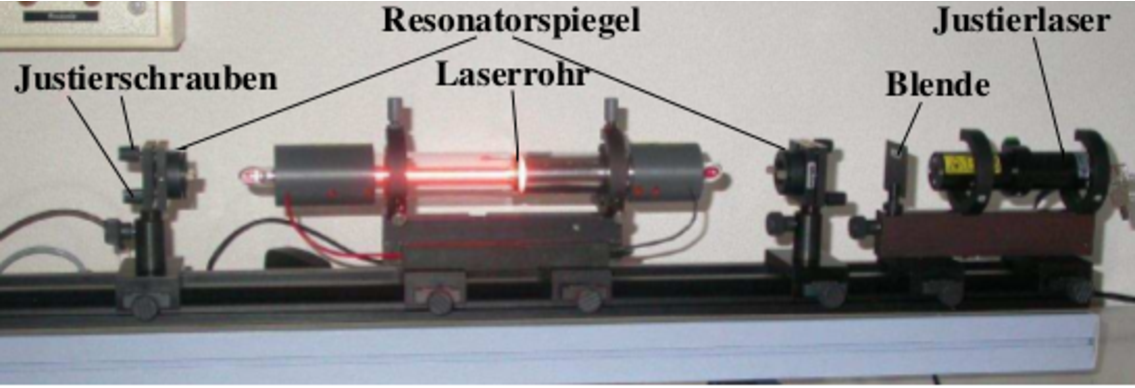
\includegraphics[scale=0.75]{../Grafiken/Aufbau.pdf}
\caption{Der Aufbau des HeNe-Lasers\cite{V61}}\label{Aufbau}
\end{figure}
\FloatBarrier
\begin{table}[h!]
\centering
\begin{tabular}{c c c}
Spiegel & Bezeichnung & Oberflächenbeschaffenheit \\\hline
plan & flat/flat & $HR$ (Hohe Reflexivität) $R\ge 99\%$\\
konkav & $r=1000$mm/flat & $HR$ (Hohe Reflexivität) $R\ge 99\%$\\
konkav & $r=1400$mm/flat & $HR$ (Hohe Reflexivität) $R\ge 99\%$\\
konkav & $r=1400$mm/flat & $OC$ (Auskopplung) $T=1.5,...1.8\% $
\end{tabular}
\caption{Die Daten der zur Verfügung Stehenden Spiegeln.\cite{V61}\label{Eigenschaften}}
\end{table}
\FloatBarrier
Für den Grundaufbau stehen verschiedene Komponenten zur Verfügung, eine optische Schiene an deren einen Ende ein Justierlaser\footnote{Mit den Eigenschaften: $\lambda=532$nm und $P_{\text{max}}=1$ mW, wobei nur die geringere Leistung $P_{\text{red}}=0,2$ mW verwendet wurde.} befestigt ist, verschiedene Spiegel, zwei Blenden mit Fadenkreuz und ein Laserrohr\footnote{Abmessungen: Länge $l=402$mm, Durchmesser $d_{\text{HeNe}}=1,1$mm} an dessen Enden die Brewster-Fenster sind.\\ 
Als erstes wird eine Blende je vor dem Justierlaser, sowie am anderen Ende der Schiene befestigt. Mithilfe der Justierschrauben am Laser wird er so ausgerichtet, dass die Beugungsringe des Justierlasers in der Mitte des Fadenkreuzes der hinteren Blende sind.\\
Als nächstes wird der teildurchlässige Spiegel mit der reflektierenden Seite zum Justierlaser gerichtet auf die schiene gestellt. Der Spiegel wird, mithilfe der Justierschrauben vom Spiegel, so eingestellt das der helle Rückreflex in der Mitte der Blende ist, die vor dem Laser steht.\\ 
Nun wird der zweite Spiegel auf der Schiene zwischen dem ersten Spiegel und der Blende, vor dem Justielaser, befestigt und mit der Reflektierenden Seite zum ersten Spiegel gewannt. Dieser Spiegel wird eingestellt wie der erste Spiegel, mit dem Unterschied das der diffuse Rückreflex in die Mitte des Fadenkreuz sein muss.\\
Nun wird das Laserrohr zwischen die Spiegel gestellt. Es ist darauf zu achten, dass der Strahl des Justierlasers mittig durch das Laserrohr führt, dazu befinden sich sechs Justierschrauben an diesem. Dazu muss der Strahl an beiden Seiten mittig durch die Brewster-Fenster geleitet werden.\\
Die Grundjustage ist damit abgeschlossen. Der Justierlaser wird nun ausgeschaltet und der eigentliche HeNe-Laser kann nun durch ein Hochspannungsgerät mit einem Strom von maximal $I=1.6$ mA betrieben werden. Jetzt wird noch kein Laserstrahl zusehen sein. Nun werden die Justierschrauben vorsichtig gedreht bis ein Strahl zwischen Laserrohr und Spiegeln zu sehen ist, wenn dies nach längerer Zeit noch nicht der Fall ist muss die Grundjustage wiederholt werden.\\
%\begin{center}
%\textbf{\textcolor{red}{Achtung! Laser der Klasse 3B,}\centering}\\ 
%\textbf{\textcolor{red}{Nicht in den Laserstrahl Blicken,}\centering}\\
%\textbf{\textcolor{red}{Schutzbrille Tragen!}\centering}
%\end{center}


\subsection{Messaufgaben}
Für die Messaufgaben werden noch weitere Komponenten benötigt wie einen Schirm, eine Photodiode, eine Mikrometerschraube, ein Gitter, Polarisationsfilter und ein Draht.
\subsubsection[TEM-Moden des Lasers]{$\mathbf{TEM}$-Moden des Lasers}
Es werden nun zwei TEM-Moden vermessen, ein mal die Grundmode TEM${}_{00}$ und die $\mathrm{TEM}_{10}$-Mode. Zur Vermessung der Moden wird hinter dem Auskoppelspiegel eine Streulinse montiert, damit der Strahl aufgefächert wird und so mit genauer vermessbar ist. Ans Ende der Schiene wird eine Photodiode auf einer Mikrometerschraube befestigt. Damit lässt sich nun der Strom, der durch die Intensität des Strahls hervorgerufen wird, vermessen, in Abhängigkeit zum Abstand zur Strahlenachse. Dbei gilt das der Strom proportional zur Intensität ist. \\
Für die $\mathrm{TEM}_{10}$-Mode wird zwischen Laserrohr und dem Auskoppelspiegel ein dünner Draht in dem Strahl montiert, dieser unterdrückt die $\mathrm{TEM}_{00}$-Mode. Hier Lässt sich wieder der Strom in Abhängigkeit zum Abstand messen.
\subsubsection{Polarisation des Lasers}
Mithilfe des Polarisationsfilters wird die Intensität in Abhängigkeit zur Polarisation gemessen. Dazu werden sowohl der Draht als auch die Linse von der Schiene genommen. Anstelle der Linse wird der Filter eingebaut.
\subsubsection{Bestimmung der Wellenlänge}

Die Wellenlänge kann mithilfe von Beugung am Gitter bestimmt werden. Dazu werden sowohl der Filter als auch die Photodiode ausgebaut und ans Ende der Schiene ein Gitter mit bekannter Gitterkonstante gestellt.
\subsubsection{Stabilität des Lasers}

Bei dieser Messung wird die Intensität in Abhängigkeit zu der Resonatorlänger gemessen. Dazu wird anstelle des Gitters wieder die Photodiode montiert. Jetzt wird die Resonatorlänge vergrößert bis zur ersten Nullstelle des Stabilitätsparameters wie in  \cref{fig:Stabilitaet} zu sehen.


